\documentclass[journal, a4paper, 12pt]{IEEEtran}

\usepackage{cite}
\usepackage{graphicx}
\usepackage{psfrag} 
\usepackage{subfigure}
\usepackage{url}
\usepackage{stfloats} 
\usepackage{amsmath}
\usepackage{colortbl}
\usepackage{xcolor}
\usepackage{tikz}
\usepackage{pgfplots}
\interdisplaylinepenalty=2500
\usepackage{array}
\usepackage{tabularx}
\usetikzlibrary{shapes}

\setlength{\parskip}{\baselineskip}%
\setlength{\parindent}{0pt}%



\renewcommand{\arraystretch}{1.35}

\begin{document}

\title{NLP Project: Authorship Detection of Twitter Tweets}
\author{Clemens Biehl, Daniel Wehner, Fabian Otto, Philipp Kapelle
\thanks{TU Darmstadt, WS 2017/2018.}}
\markboth{Natural Language Processing and the Web}{}
\maketitle

\begin{abstract}
In our project we worked on the authorship detection of Twitter tweets. This report gives a short summary of the results which we could produce during the project.
\end{abstract}
	
\section{Introduction and Research Problem}
Millions of texts and posts are published on social media platforms such as Twitter or Facebook every day. The identification of the authorship is often a crucial task in Natural Language Processing. This might be helpful when checking the authenticity of a post. In this project we therefore aim to classify Twitter Tweets to identify the authors of the tweets and try to answer the following questions:
\vspace{-2mm}
\begin{itemize}
\item Which types of writing-style features are effective for identifying the authorship of online messages?
\item Which classifiers perform best for identifying the authorship of online messages?
\item To what extent can authorship-identification techniques be applied to online messages across different genres such as politics or sports?
\end{itemize}
\vspace{-2mm}
To answer these questions we tried various combinations of features, classifiers and genres such as politics and sports and evaluated these combinations.


\section{Twitter Crawler}
In order to fulfill our research problem, we have to acquire many tweets that have been written by a single author in the english language. Therefor we need to identify Twitteraccounts, that are operated by a single user and have a large amount of original tweets. To find these Twitteraccounts, data from https://www.socialbakers.com has been analyzed. 

The site lists the most followed Twitteraccounts grouped by country of the user and his/her profession (e.g. Actor, UK). However, it does not distinguish between how many people operate the Twitteraccount, nor how many tweets have been written. Still one can assume that a Twitteraccount that is among the most followed accounts worldwide, is named after a single Person, is verified, contains a lot of personal information including original pictures of said person and does not state that it is operated by another person, contains a large amount of original tweets. 

Therefor the list provided by the website has been the primary source of the data used. The Twitteraccounts selected have been identified by the following steps. First four fields of profession have been selected ('Actor', 'Broadcast Star', 'Politics', 'Sport Star') due to a high densitiy of single-author accounts. To get reliable english language tweets, USA and United Kingdom have been selected as the only two possible countries of origin. Also to get a fair distribution between american english and british english the top twelve accounts per country will be added as potential accounts to be crawled. 

Twitter users have a timeline that provides all Tweets, Retweets and information about the account itself, such as total amount of Tweets tweeted. In this amount Retweets are counted as Tweets. During the process of identification the goal was set to get at least 20 distinct authors per category with at least 1000 original tweets each and an about equal distribution between US and UK citizens. Since the only information on the amount of tweets a user has sent includes Retweets, which contain text the user hasn't written, accounts with less than 3000 Tweets in total have been filtered out. Finally an extra category of Twitteraccounts with less tweets and possibly not only english language tweets has been added with selected accounts that may be interesting ('FunMix'). 

After the accounts have been identified, each of them has been reviewed and determined, whether or not it is likely, that it is run by a single user. Also the total amount of tweets has been checked. Disqualified accounts then have been replaced by the next Twitteraccount from the list provided by https://www.socialbakers.com, that fulfills the requirements.

The list of users has been stored in a JSON file containing the names, countries and Twitterhandles of the users. This JSON file was then read by the Twittercrawler, and each user's timeline requested from Twitter using the TwitterAPI and the Java library 'twitter4j'. 

The timeline is divided into pages containing up to 100 Tweets, that each have to be requested individually. To limit the traffic and optimize the data output, a single page was requested, filtered locally for original tweets only and checked, if the 1000 Tweets were reached. If not, the process was repeated, which is the reason for minor differences between the amount of Tweets per user. At the end of the crawling step, all Tweets were saved as JSON files. 

In total 100 Twitteraccounts have been identified and crawled, resulting in 1000 to 1099 (mean 1043) original tweets per author.  



\section{Data Provisioning}
\label{sec:provisioning}
\vspace{-2mm}
As already mentioned, Twitter will be the source for the data to be analyzed. We focused on tweets of 20 famous politicians, sportsmen, actors and broadcast stars of the English-speaking world since we confined ourselves to english tweets. For instance, we collected tweets from the following accounts of politicians:

\footnotesize
\textit{
realDonaldTrump, BarackObama, ChuckGrassley, RepJaredPolis, BorisJohnson, clairecmc, ChrisChristie, jahimes, jeremycorbyn, CarolineLucas, David\_Cameron, BernieSanders, RonPaul, SpeakerRyan, mike\_pence, DavidLammy, timfarron, Ed\_Miliband, ChukaUmunna, tom\_watson
}
\normalsize

The number of politicians' tweets collected per account is 1,000, which makes 20,000 tweets in total. When guessing the authors randomly, we would get an accuracy of approximaltey 5\,\% (since the training data consists of tweets from 20 different authors). This is our baseline. We should have an accuracy better than 5\,\%.

\begin{figure}
\caption{JSON representation of a tweet written by Barack Obama that was crawled from Twitter}
\tiny
\begin{verbatim}
{  
   "in_reply_to_status_id_str":null,
   "in_reply_to_status_id":null,
   "coordinates":null,
   "created_at":"Mon Jan 15 14:46:02 +0000 2018",
   "truncated":false,
   "in_reply_to_user_id_str":null,
   "source":"<a href=\"http://twitter.com/download/
     iphone\" rel=\"nofollow\">Twitter for
     iPhone<\/a>",
   "retweet_count":367963,
   "retweeted":false,
   "geo":null,
   "in_reply_to_screen_name":null,
   "is_quote_status":false,
   "entities":{  
      "urls":[  

      ],
      "hashtags":[  

      ],
      "user_mentions":[  

      ],
      "symbols":[  

      ]
   },
   "full_text":"Dr. King was 26 when the Montgomery
      bus boycott began. He started small, rallying
      others who believed their efforts mattered,
      pressing on through challenges and
      doubts to change our world (...)",
   "id_str":"952914779458424832",
   "in_reply_to_user_id":null,
   "display_text_range":[  
      0,
      279
   ],
   "favorite_count":1393878,
   "id":952914779458424832,
   "place":null,
   "contributors":null,
   "lang":"en",
   "user":{  
      "id_str":"813286",
      "id":813286
   },
   "favorited":false
}
\end{verbatim}
\normalsize
\end{figure}

\section{Pipeline}
\label{sec:pipeline}
The general process for the authorship identification follows a usual NLP pipeline approach as depicted in Figure 2. The single steps will be described further in the following sections. The \textit{Data Provisiong} was described in the last section. The preprocessing depends on the features which are used, e.\,g. the contextuality measure requires part-of-speech tagging.

\begin{figure}[h]
	\caption{Visualization of the pipeline built for the authorship identification. After providing the data by the crawler, the data is
	 preprocessed. The feature extraction phase takes care of creating useful features for classification for the training of the model.
	The last step is the evaluation of the model.}
	\vspace*{5mm}
	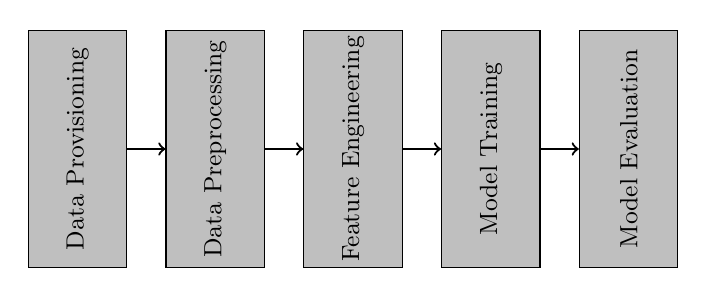
\begin{tikzpicture}
		\small
		\node[rectangle,fill=lightgray,draw=black,minimum height=3cm, minimum width=1.25cm] (A) at (0,0) {};
		\node[rectangle,fill=lightgray,draw=black,minimum height=3cm, minimum width=1.25cm] (B) at (1.75,0) {};
		\node[rectangle,fill=lightgray,draw=black,minimum height=3cm, minimum width=1.25cm] (C) at (3.5,0) {};
		\node[rectangle,fill=lightgray,draw=black,minimum height=3cm, minimum width=1.25cm] (D) at (5.25,0) {};
		\node[rectangle,fill=lightgray,draw=black,minimum height=3cm, minimum width=1.25cm] (E) at (7,0) {};

		\draw[thick,->] (A) -- (B);
		\draw[thick,->] (B) -- (C);
		\draw[thick,->] (C) -- (D);
		\draw[thick,->] (D) -- (E);

		\node[rotate=90] at (0,0) {Data Provisioning};
		\node[rotate=90] at (1.75,0) {Data Preprocessing};
		\node[rotate=90] at (3.5,0) {Feature Engineering};
		\node[rotate=90] at (5.25,0) {Model Training};
		\node[rotate=90] at (7,0) {Model Evaluation};
	\end{tikzpicture}
\end{figure}

\textbf{Data Provisioning}: For information see section \ref{sec:provisioning}

\textbf{Feature Engineering}: Please see section \ref{sec:features}

\textbf{Model Training and Evaluation}: Please refer to section \ref{sec:training-eval} 

\section{Feature Engineering}
\label{sec:features}

The feature engineering phase is crucial for the success of the project since the performance of the classifiers depends significantly on the quality of the features used. Table \ref{tab:features} summarizes the features which we have taken into account when training the classifiers.

\begin{table}[!hbt]
	\begin{center}
		\caption{List of features which were considered for training the classifiers.}
		\label{tab:features}
		\begin{tabularx}{80mm}{| l | X |}
			\hline
			\rowcolor{lightgray}
			\textbf{Feature}			& \textbf{Explanation}						\\ \hline\hline
			Total number of chars		& How long is the tweet						\\ \hline
			Emoticon ratio		  	& Proportion of emoticons in the text. 			\\ \hline
			Number of hashtags		& How many hashtags are used in the tweet. 	\\ \hline
			Word frequencies        	& Which words are used frequently 				\\ \hline
			Lexical diversity			& How rich is the vocabulary of the author? 		\\ \hline
			Contextuality Measure		& Score between 0 and 100
								  	(0 very context dependent = many pronouns, adverbs, ...;
									100 not content dependent = many nouns, ...) 
																				\\ \hline
			Exclamation Ratio			& How many exclamation marks are used?		\\ \hline
			Superlative Ratio			& Proportion of superlatives in the tweet?		\\ \hline
			PastVsFuture				& Ratio of verbs in past tense/present tense		\\ \hline
			\hline
		\end{tabularx}
	\end{center}
\end{table}

With emoticons playing a central role in social media they represent a good feature to consider. Therefore, the emoticon ratio (ER) is calculated (the number of tokens which represent emoticons divided by the total number of tokens in the text).

Other features like sentence features did not perform well since twitter texts are very short.

\begin{equation}
	\text{ER} = \frac{\text{\# of emoticon tokens}}{\text{\# of tokens}}
\end{equation}

Also very characteristic for specific authors is the number of hashtags they use when writing a tweet, the word frequencies (does the author prefer specific words over other words) and the lexical diversity (also known as type-token ratio [TTR] which analyzes how many different words are used in the tweet)

\begin{equation}
\text{TTR} = \frac{V(N)}{N}
\end{equation}

Other measures for lexical diversity/vocabulary richness:
\small
\begin{equation}
\text{Yule's $K$} = C \left[ -\frac{1}{N} + \sum_{m=1}^{m_{max}} V(m,N)\left(\frac{m}{N}\right)^2 \right]
\end{equation}

\begin{equation}
\text{Simpson's $D$} = \sum_{m=1}^{m_{max}} V(m,N)\frac{m}{N}\frac{m-1}{N-1}
\end{equation}

\begin{equation}
\text{Herdan $V_m$} = \sqrt{\sum_{m=1}^{m_{max}}V(m,N)\left(\frac{m}{N}\right)^2-\frac{1}{V(N)}} 
\end{equation}

\begin{equation}
\text{Sichel's $S$} = \frac{V(1,N)}{V(N)}
\end{equation}

\begin{equation}
\text{Honore's $R$} = 100 \frac{\log \left(N\right)}{1 - \frac{V(1,N)}{V(N)}}
\end{equation}

\begin{equation}
\text{Brunet's $W$} = N^{V - c} \quad \text{usually $c = 0.17$}
\end{equation}

\begin{equation}
\text{Uber Index} = \frac{\log\left(N\right)^2}{\log \left(N\right) - \log \left(V(N)\right)}
\end{equation}

\begin{tabular}{@{}>{$}l<{$}l@{}}
	N	 		& Length of text \\ 
 	V(N) 		& Size of vocabulary \\
    	V(m,N) 		& Number of words in $N$ occuring $m$ times \\
	V(1,N) 		& Number of \textbf{Hapax Legomena} \\
	V(2,N) 		& Number of \textbf{Hapax Dislegomena} \\
    	m_{max}	& maximal frequency
\end{tabular}

\normalsize
Another feature of interest is the contextuality measure which indicates how context-dependent a text is. The contextuality measure produces values between 0 and 100. A value of 0 indicates a very context-dependent text which contains many pronouns, adverbs, etc. The higher the value the less context-dependent the text is (the text is then said to be \textit{formal} as opposed to \textit{contextual}). This is the formula which computes the score:

\begin{equation}
\small
F = \frac{n + a + p + d - pr - v - ad - if + 100}{2}
\end{equation}

\begin{tabular}{@{}>{$}l<{$}l@{}}
    n 		& noun frequency \\
    a 		& adjective frequency \\
    p 		& preposition frequency \\
    d 		& determiner frequency \\
    pr		& pronoun frequency \\
    v			& verb frequency \\
    ad		& adverb frequency \\
    if			& interjection frequency \\	
\end{tabular}

\enlargethispage{\baselineskip}
\section{Evaluation}
\label{sec:training-eval}

As a basis we used the \texttt{WekaTwitterSentimentDemo} which we found in the DKPro\,TC GitHub Repository resulting in an accuracy of approximately $13\,\%_{\text{Naive Bayes}}$, approximately $8.5\,\%_{\text{Random Forest}}$ and approximately $8\,\%_{\text{Logistic}}$ (Used features in the demo: EmoticonRate and Number of Hashtags, Number of Tokens per Sentence). We used this as the baseline and added further features. The evaluation is based on a test set of 10\% of the tweets per genre. The results for different features and classifiers are summarized in tables \ref{tab:results-nb} (\textbf{Naive Bayes}),  \ref{tab:results-rf} (\textbf{Random Forest}) and \ref{tab:results-logistic} (\textbf{Logistic Regression}) and in figures \ref{fig:results-nb} (\textbf{Naive Bayes}), \ref{fig:results-rf} (\textbf{Random Forest}) and \ref{fig:results-logistic} (\textbf{Logistic Regression}) respectively.

\begin{table}[!hbt]
	\begin{center}
		\caption{Evaluation results for different feature setups ordered by increasing accuracy. Classifier = \textbf{Naive Bayes}}
		\label{tab:results-nb}
		\begin{tabularx}{80mm}{| l | X | r |}
			\hline
			\rowcolor{lightgray}
			\multicolumn{3}{| c |}{\textbf{Naive Bayes}} 									\\ \hline
			\rowcolor{lightgray}
			\textbf{Nr.}		&	\textbf{Setup}					& \textbf{Accuracy}		\\ \hline\hline
			1			&	\texttt{WekaTwitterSentimentDemo}	& \textbf{12.88\,\%}		\\ \hline
			2			&	TTR 	(Type-Token-Ratio)			& \textbf{13.48\,\%}		\\ \hline
			3			&	TTR + Contextuality Measure			& \textbf{16.60\,\%}		\\ \hline
			4			&	TTR + UpperCase + Alphabetic + Digits + WhiteSpaces + TabSpaces
																& \textbf{16.59\,\%}		\\ \hline
			5			& 	TTR + Contextuality Measure + Exclamation Ratio
																& \textbf{19.25\,\%}		\\ \hline
			6			&	TTR + Contextuality Measure + Exclamation Ratio + Superlative Ratio
																& \textbf{18.19\,\%}		\\ \hline
			7			&	TTR + Contextuality Measure + Exclamation Ratio + PastVsFuture
																& \textbf{19.38\,\%}		\\ \hline
			8			&	TTR + Contextuality Measure + Exclamation Ratio + PastVsFuture + Avg Nr of Chars per Sentence
																& \textbf{20.22\,\%}		\\ \hline
			9			&	TTR + Contextuality Measure + Exclamation Ratio + PastVsFuture + Avg Nr of Chars per Sentence + Avg Nr of Chars per Token + Nr of Chars + Nr of Sentences + Nr of Tokens
																& \textbf{19.90\,\%}		\\ \hline
			10			&	TTR + Contextuality Measure + Exclamation Ratio + PastVsFuture + Avg Nr of Chars per Sentence + UpperCase + Alphabetic + Digits + WhiteSpaces + TabSpaces
																& \textbf{21.06\,\%}		\\ \hline
			11			&	TTR + Contextuality Measure + Exclamation Ratio + PastVsFuture + Avg Nr of Chars per Sentence + UpperCase + Alphabetic + Digits + WhiteSpaces + TabSpaces + Yule's $K$ + Herdan $V_m$
																& \textbf{21.19\,\%}		\\ \hline
			12			&	TTR + Contextuality Measure + Exclamation Ratio + PastVsFuture + Avg Nr of Chars per Sentence + UpperCase + Alphabetic + Digits + WhiteSpaces + TabSpaces + N-Grams (up to trigrams)
																& \textbf{40.26\,\%}		\\ \hline
			13		&	TTR + Contextuality Measure + Exclamation Ratio + PastVsFuture + Avg Nr of Chars per Sentence + UpperCase + Alphabetic + Digits + WhiteSpaces + TabSpaces + N-Grams (up to trigrams) + POS N-Grams (up to trigrams)
																& \textbf{41.20\,\%}		\\ \hline
			14		&	TTR + Contextuality Measure + Exclamation Ratio + PastVsFuture + Avg Nr of Chars per Sentence + UpperCase + Alphabetic + Digits + WhiteSpaces + TabSpaces + N-Grams (up to trigrams) + POS N-Grams (up to trigrams) + SpellingErrorRatio
																& \textbf{41.20\,\%}		\\ \hline
			\hline
		\end{tabularx}
	\end{center}
\end{table}

% Bar diagram which visualizes the results of the different setups
\begin{figure}[!hbt]
	\begin{center}
		\caption{Evaluation results for different feature setups. Results for \textbf{Naive Bayes} classifier}
		\label{fig:results-nb}
		\vspace{5mm}
		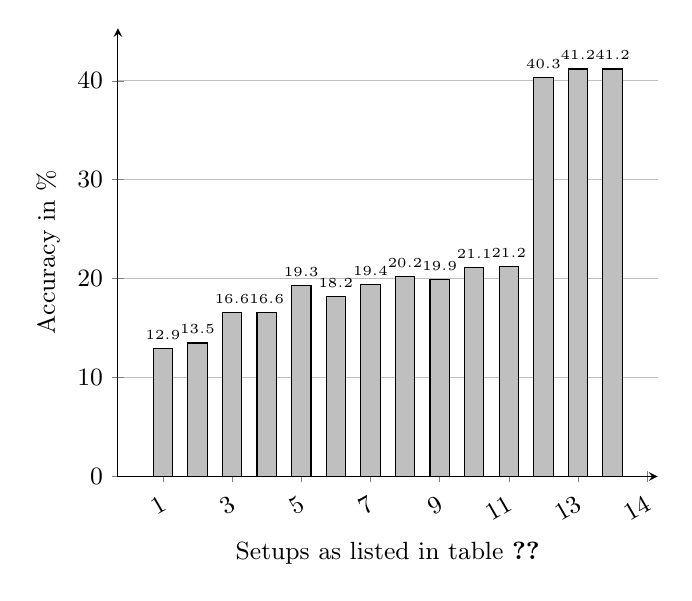
\begin{tikzpicture}
			\small
			\begin{axis}[
    				ybar, bar width=7pt,
				nodes near coords, nodes near coords align=above, point meta=rawy,
 				axis x line=bottom, axis y line=left, ymajorgrids=true,
				ylabel=$\mathrm{Accuracy\ in\ \%}$, ymin=0, ytick={0,10,20,30,40,50,60,70,80,90,100},
				enlargelimits=auto,
    				xlabel=Setups as listed in table \ref{tab:results-nb}, symbolic x coords={1,2,3,4,5,6,7,8,9,10,11,12,13,14},
    				x tick label style={rotate=30,anchor=north east},
    			]
    			
    				\addplot[fill=lightgray,font=\tiny] coordinates {
      					(1,12.9)
      					(2,13.5)
						(3,16.6)
						(4,16.6)
						(5,19.3)
						(6,18.2)
						(7,19.4)
						(8,20.2)
						(9,19.9)
						(10,21.1)
						(11,21.2)
						(12,40.3)
						(13,41.2)
						(14,41.2)
    				};
  			\end{axis}
		\end{tikzpicture}
	\end{center}
\end{figure}

\begin{table}[!hbt]
	\begin{center}
		\caption{Evaluation results for different feature setups ordered by increasing accuracy.
		Classifier = \textbf{Random Forests}}
		\label{tab:results-rf}
		\begin{tabularx}{80mm}{| l | X | r |}
			\hline
			\rowcolor{lightgray}
			\multicolumn{3}{| c |}{\textbf{Random Forest}} 								\\ \hline
			\rowcolor{lightgray}
			\textbf{Nr.}		&	\textbf{Setup}					& \textbf{Accuracy}		\\ \hline\hline
			1			&	\texttt{WekaTwitterSentimentDemo}	& \textbf{8.49\,\%}		\\ \hline
			2			&	TTR (Type-Token-Ratio)				& \textbf{8.49\,\%}		\\ \hline
			3			&	TTR + Contextuality Measure			& \textbf{8.49\,\%}		\\ \hline
			4			&	TTR + UpperCase + Alphabetic + Digits + WhiteSpaces + TabSpaces
																& \textbf{95.02\,\%}		\\ \hline
			5			& 	TTR + Contextuality Measure + Exclamation Ratio
																& \textbf{8.49\,\%}		\\ \hline
			6			&	TTR + Contextuality Measure + Exclamation Ratio + Superlative Ratio + PastVsFuture 
																& \textbf{8.49\,\%}		\\ \hline
			7			&	TTR + Contextuality Measure + Exclamation Ratio + Superlative Ratio 
																& \textbf{8.49\,\%}		\\ \hline
			8			&	TTR + Contextuality Measure + Exclamation Ratio + Superlative Ratio +
							Nr of Tokens + Character Features + N-Grams
																& \textbf{95.08\,\%}		\\ \hline
			9			&	TTR + Contextuality Measure + Exclamation Ratio + Superlative Ratio +
							Nr of Tokens + Character Features + N-Grams + POS-NGrams
																& \textbf{95.03\,\%}		\\ \hline
			\hline
		\end{tabularx}
	\end{center}
\end{table}

% Bar diagram which visualizes the results of the different setups
\begin{figure}[!h]
	\begin{center}
		\caption{Evaluation results for different feature setups. Results for \textbf{Random Forest} classifier}
		\label{fig:results-rf}
		\vspace{5mm}
		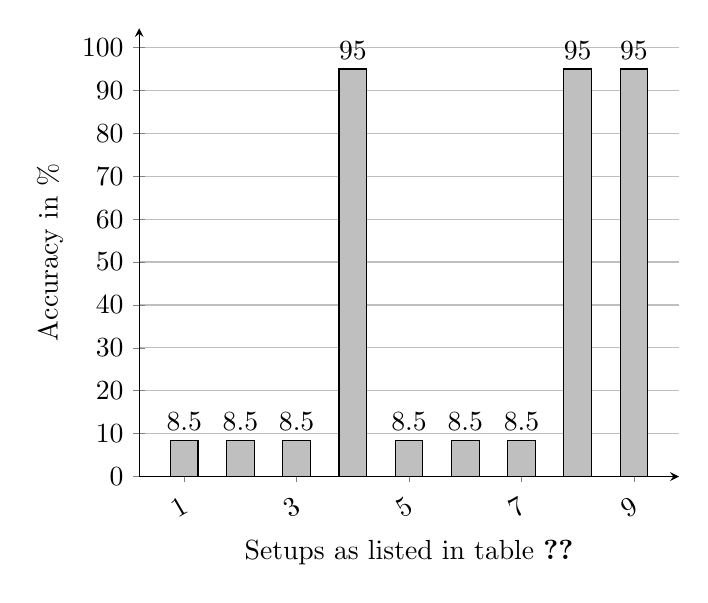
\begin{tikzpicture}
			\begin{axis}[
    				ybar, bar width=10pt,
				nodes near coords, nodes near coords align=above, point meta=rawy,
 				axis x line=bottom, axis y line=left, ymajorgrids=true,
				ylabel=$\mathrm{Accuracy\ in\ \%}$, ymin=0, ytick={0,10,20,30,40,50,60,70,80,90,100},
				enlargelimits=auto,
    				xlabel=Setups as listed in table \ref{tab:results-rf}, symbolic x coords={1,2,3,4,5,6,7,8,9},
    				x tick label style={rotate=30,anchor=north east},
    			]

    				\addplot[fill=lightgray] coordinates {
      					(1,8.5)
      					(2,8.5)
					(3,8.5)
					(4,95)
					(5,8.5)
					(6,8.5)
					(7,8.5)
					(8,95)
					(9,95)
    				};
  			\end{axis} 
		\end{tikzpicture}
	\end{center}
\end{figure}

\begin{table}[!hbt]
	\begin{center}
		\caption{Evaluation results for different feature setups ordered by increasing accuracy.
		Classifier = \textbf{Logistic Regression}}
		\label{tab:results-logistic}
		\begin{tabularx}{80mm}{| l | X | r |}
			\hline
			\rowcolor{lightgray}
			\multicolumn{3}{| c |}{\textbf{Logistic Regression}} 								\\ \hline
			\rowcolor{lightgray}
			\textbf{Nr.}		&	\textbf{Setup}					& \textbf{Accuracy}		\\ \hline\hline
			1			&	\texttt{WekaTwitterSentimentDemo}	& \textbf{7.96\,\%}		\\ \hline
			2			&	TTR (Type-Token-Ratio)				& \textbf{7.96\,\%}		\\ \hline
			3			&	TTR + Contextuality Measure			& \textbf{7.96\,\%}		\\ \hline
			4			&	TTR + UpperCase + Alphabetic + Digits + WhiteSpaces + TabSpaces
																& \textbf{20.20\,\%}		\\ \hline
			5			& 	TTR + Contextuality Measure + Exclamation Ratio
																& \textbf{7.96\,\%}		\\ \hline
			6			&	TTR + Contextuality Measure + Exclamation Ratio + Superlative Ratio + PastVsFuture 
																& \textbf{7.96\,\%}		\\ \hline
			7			&	TTR + Contextuality Measure + Exclamation Ratio + Superlative Ratio 
																& \textbf{7.96\,\%}		\\ \hline
			8			&	TTR + Contextuality Measure + Exclamation Ratio + Superlative Ratio +
							Nr of Tokens + Character Features + N-Grams
																& \textbf{20.20\,\%}		\\ \hline
			9			&	TTR + Contextuality Measure + Exclamation Ratio + Superlative Ratio +
							Nr of Tokens + Character Features + N-Grams + POS-NGrams
																& \textbf{20.20\,\%}		\\ \hline
			\hline
		\end{tabularx}
	\end{center}
\end{table}

% Bar diagram which visualizes the results of the different setups
\begin{figure}[!h]
	\begin{center}
		\caption{Evaluation results for different feature setups. Results for \textbf{Logistic Regression} classifier}
		\label{fig:results-logistic}
		\vspace{5mm}
		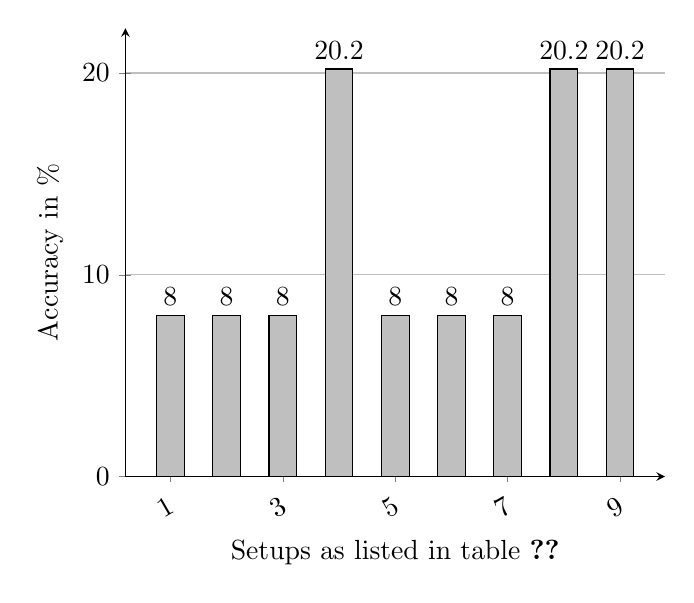
\begin{tikzpicture}
			\begin{axis}[
    				ybar, bar width=10pt,
				nodes near coords, nodes near coords align=above, point meta=rawy,
 				axis x line=bottom, axis y line=left, ymajorgrids=true,
				ylabel=$\mathrm{Accuracy\ in\ \%}$, ymin=0, ytick={0,10,20,30,40,50,60,70,80,90,100},
				enlargelimits=auto,
    				xlabel=Setups as listed in table \ref{tab:results-rf}, symbolic x coords={1,2,3,4,5,6,7,8,9},
    				x tick label style={rotate=30,anchor=north east},
    			]

    				\addplot[fill=lightgray] coordinates {
      					(1,8.0)
      					(2,8.0)
					(3,8.0)
					(4,20.20)
					(5,8.0)
					(6,8.0)
					(7,8.0)
					(8,20.20)
					(9,20.20)
    				};
  			\end{axis} 
		\end{tikzpicture}
	\end{center}
\end{figure}

\section{Deep Learning}

Extracting the features is very tedious and it is more or less a trial and error process. There are many combinations of features that have to be taken into account and which have to be evaluated. A remedy for that is for example a \textbf{Deep Learning} approach. Such approaches have become very famous recently and also for Natural Language Processing there are several application areas for such methods. Deep Learning is capable of automating this combersome process by making use of several layers that are responsible for feature extraction and transformation. The results of one layer represent the input of the next layers. Very often \textbf{Artificial Neural Networks (ANN)} are used in such cases.

\begin{figure}[h]
	\caption{A simple neural network with two hidden layers.}
	\centering
	\vspace{5mm}
	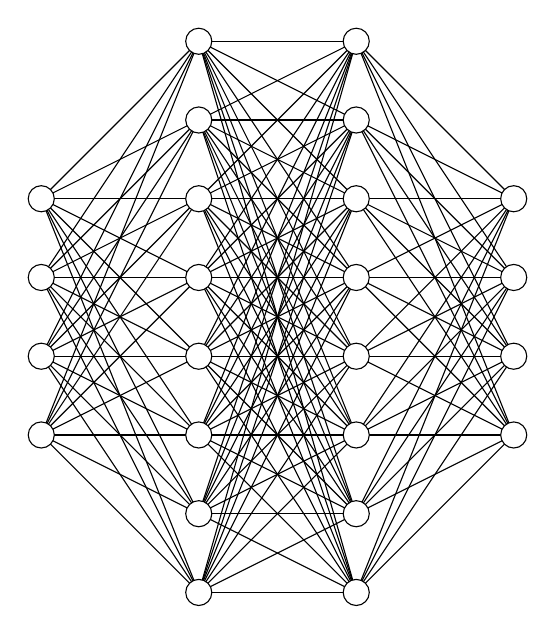
\begin{tikzpicture}
		\foreach \y in {1, 2, 3, 4, 5, 6, 7, 8}{
			\draw (0,3) -- (2,\y);
			\draw (0,4) -- (2,\y);
			\draw (0,5) -- (2,\y);
			\draw (0,6) -- (2,\y);
		}

		\foreach \y in {1, 2, 3, 4, 5, 6, 7, 8}{
			\draw (2,1) -- (4,\y);
			\draw (2,2) -- (4,\y);
			\draw (2,3) -- (4,\y);
			\draw (2,4) -- (4,\y);
			\draw (2,5) -- (4,\y);
			\draw (2,6) -- (4,\y);
			\draw (2,7) -- (4,\y);
			\draw (2,8) -- (4,\y);
		}
		
		\foreach \y in {1, 2, 3, 4, 5, 6, 7, 8}{
			\draw (4,\y) -- (6,3);
			\draw (4,\y) -- (6,4);
			\draw (4,\y) -- (6,5);
			\draw (4,\y) -- (6,6);
		}

		\foreach \y in {3, 4, 5, 6}
			\node[circle,draw=black,fill=white] at (0,\y) {};
		\foreach \y in {1, 2, 3, 4, 5, 6, 7, 8}
			\node[circle,draw=black,fill=white] at (2,\y) {};
		\foreach \y in {1, 2, 3, 4, 5, 6, 7, 8}
			\node[circle,draw=black,fill=white] at (4,\y) {};
		\foreach \y in {3, 4, 5, 6}
			\node[circle,draw=black,fill=white] at (6,\y) {};
	\end{tikzpicture}
\end{figure}

\section{Component Diagram}

\section{Conclusion}
The experiments showed that character-based linguistic style features such as the frequencies of upper case, alphabetic, digit and white- and tabspace characters are good indicators for an author's style in writing tweets. Likewise the Contextuality Measure and PastVsFuture features increased accuracy. In contrast, sentence-based features such as the number of sentences or the average number of characters in a sentence decreased accuracy, which can be explained by the general brevity of tweets and the fact that tweets often do not include clear sentence boundaries. Some of the measures for lexical diversity/vocabulary richness did not contribute to the accuracy, therefore only Yule's $K$ and Herdan $V_m$ were used. Using N-Grams and Part-of-Speech N-Grams significantly improved the accuracy, presumably because they incorporate the author's specific vocabulary.\\
The final accuracy of 95.08\% using a random forest classifier and the features shown in table III (column 8) is remarkably high for the task of authorship identification and might not generalize well to other domains, since the N-Grams are very specific with respect to the training data.\\
Future experiments will have to investigate if the features used here can be applied in and across different domains. Furthermore, deep learning has to be considered for including an implicit feature extraction in the classifier training.

\begin{thebibliography}{2}

	\bibitem{Zheng06}
	Zheng, Rong and Li, Jiexun and Chen, Hsinchun and Huang, Zan. A Framework for Authorship Identification
	of Online Messages: Writing-Style Features and Classification Techniques. {\em Journal of the American
	Society for Information Science and Technology},
	vol.~57, no.~3, pp.~378-393, 2006.

	\bibitem{Hout07}
	Hout, Roeland and Vermeer, Anne. Comparing measures of lexical richness. {\em Modelling and assessing vocabulary 
	knowledge}, pp.~93-116, 2007.

	\bibitem{Fissette10}
	Fissette, Marcia. Author identification in short texts. 2010.

	\bibitem{Green13}
	Green, Rachel M. and Sheppard, John W. Comparing Frequency- and Style-Based Features for Twitter
	Author Identification. {\em AAAI Press}, 2013.
	
	\bibitem{Heylighen02}
	Heylighen, Francis; Dewaele, Jean-Marc. Variation in the Contextuality of Language: An Empirical Measure.
	{\em Foundations of Science}, vol.~7, no.~3, pp.~293-340, September 2002.

	\bibitem{Aihara15}
	Tanaka-Ishii, Kumiko and Aihara, Shunsuke. Computational Constancy Measures of Texts—Yule's K and Rényi's Entropy.
	{\em Computational Linguistics} vol.~41, no.~3, pp.~481-502, September 2015.

	\bibitem{Tweedie98}
	Tweedie, Fiona J. and BaayenHow, R. Harald. Variable May a Constant be? Measures of Lexical Richness in Perspective.
	{\em Computers and the Humanities} vol.~32, no.~5, pp.~323-352, September 1998.	

	\bibitem{Bhatia}
	Bhatia Archna et al. TweetNLP, Carnegie Mellon. \url{http://www.cs.cmu.edu/~ark/TweetNLP}

\end{thebibliography}

\end{document}